\documentclass[11pt]{article}
\usepackage{amsmath,amssymb,amsmath,amsthm,amsfonts}
\usepackage{latexsym,graphicx}
\usepackage{fullpage,color}
\usepackage{url,hyperref}
\usepackage{natbib}
\usepackage{graphicx,subfigure}
\usepackage{algorithm}
\usepackage{algorithmic}
\usepackage{listings}
\usepackage{xcolor}
\usepackage{color}

\numberwithin{equation}{section}

\pagestyle{plain}

\setlength{\oddsidemargin}{0in}
\setlength{\topmargin}{0in}
\setlength{\textwidth}{6.5in}
\setlength{\textheight}{8.5in}

\newtheorem{fact}{Fact}[section]
\newtheorem{question}{Question}[section]
\newtheorem{lemma}{Lemma}[section]
\newtheorem{theorem}[lemma]{Theorem}
\newtheorem{assumption}[lemma]{Assumption}
\newtheorem{corollary}[lemma]{Corollary}
\newtheorem{prop}[lemma]{Proposition}
\newtheorem{claim}{Claim}[section]
\newtheorem{remark}{Remark}[section]
\newtheorem{definition}{Definition}[section]
\newtheorem{prob}{Problem}[section]
\newtheorem{conjecture}{Conjecture}[section]
\newtheorem{property}{Property}[section]

\def\A{{\bf A}}
\def\a{{\bf a}}
\def\B{{\bf B}}
\def\bb{{\bf b}}
\def\C{{\bf C}}
\def\c{{\bf c}}
\def\D{{\bf D}}
\def\d{{\bf d}}
\def\E{{\bf E}}
\def\e{{\bf e}}
\def\F{{\bf F}}
\def\f{{\bf f}}
\def\g{{\bf g}}
\def\h{{\bf h}}
\def\G{{\bf G}}
\def\H{{\bf H}}
\def\I{{\bf I}}
\def\K{{\bf K}}
\def\k{{\bf k}}
\def\LL{{\bf L}}
\def\M{{\bf M}}
\def\m{{\bf m}}
\def\N{{\bf N}}
\def\n{{\bf n}}
\def\PP{{\bf P}}
\def\Q{{\bf Q}}
\def\q{{\bf q}}
\def\R{{\bf R}}
\def\rr{{\bf r}}
\def\S{{\bf S}}
\def\s{{\bf s}}
\def\T{{\bf T}}
\def\tt{{\bf t}}
\def\U{{\bf U}}
\def\u{{\bf u}}
\def\V{{\bf V}}
\def\v{{\bf v}}
\def\W{{\bf W}}
\def\w{{\bf w}}
\def\X{{\bf X}}
\def\x{{\bf x}}
\def\Y{{\bf Y}}
\def\y{{\bf y}}
\def\Z{{\bf Z}}
\def\z{{\bf z}}
\def\0{{\bf 0}}
\def\1{{\bf 1}}



\def\AM{{\mathcal A}}
\def\CM{{\mathcal C}}
\def\DM{{\mathcal D}}
\def\EM{{\mathcal E}}
\def\GM{{\mathcal G}}
\def\FM{{\mathcal F}}
\def\IM{{\mathcal I}}
\def\JM{{\mathcal J}}
\def\KM{{\mathcal K}}
\def\LM{{\mathcal L}}
\def\NM{{\mathcal N}}
\def\OM{{\mathcal O}}
\def\PM{{\mathcal P}}
\def\SM{{\mathcal S}}
\def\TM{{\mathcal T}}
\def\UM{{\mathcal U}}
\def\VM{{\mathcal V}}
\def\WM{{\mathcal W}}
\def\XM{{\mathcal X}}
\def\YM{{\mathcal Y}}
\def\RB{{\mathbb R}}
\def\RBmn{{\RB^{m\times n}}}
\def\EB{{\mathbb E}}
\def\PB{{\mathbb P}}


\def\alp{\mbox{\boldmath$\alpha$\unboldmath}}
\def\bet{\mbox{\boldmath$\beta$\unboldmath}}
\def\epsi{\mbox{\boldmath$\epsilon$\unboldmath}}
\def\etab{\mbox{\boldmath$\eta$\unboldmath}}
\def\ph{\mbox{\boldmath$\phi$\unboldmath}}
\def\pii{\mbox{\boldmath$\pi$\unboldmath}}
\def\Ph{\mbox{\boldmath$\Phi$\unboldmath}}
\def\Ps{\mbox{\boldmath$\Psi$\unboldmath}}
\def\ps{\mbox{\boldmath$\psi$\unboldmath}}
\def\tha{\mbox{\boldmath$\theta$\unboldmath}}
\def\Tha{\mbox{\boldmath$\Theta$\unboldmath}}
\def\muu{\mbox{\boldmath$\mu$\unboldmath}}
\def\Si{\mbox{\boldmath$\Sigma$\unboldmath}}
\def\si{\mbox{\boldmath$\sigma$\unboldmath}}
\def\Gam{\mbox{\boldmath$\Gamma$\unboldmath}}
\def\Lam{\mbox{\boldmath$\Lambda$\unboldmath}}
\def\De{\mbox{\boldmath$\Delta$\unboldmath}}
\def\Ome{\mbox{\boldmath$\Omega$\unboldmath}}
\def\Pii{\mbox{\boldmath$\Pi$\unboldmath}}
\def\varepsi{\mbox{\boldmath$\varepsilon$\unboldmath}}

\def\argmax{\mathop{\rm argmax}}
\def\argmin{\mathop{\rm argmin}}
\def\bias{\mathsf{bias}}
\def\var{\mathsf{var}}
\def\sgn{\mathsf{sgn}}
\def\tr{\mathsf{tr}}
\def\rk{\mathrm{rank}}
\def\poly{\mathrm{poly}}
\def\diag{\mathsf{diag}}
\def\st{\mathsf{s.t.}}

\newcommand{\red}[1]{{\color{red}#1}}



\lstset{ %
extendedchars=false,            % Shutdown no-ASCII compatible
language=Python,                % choose the language of the code
xleftmargin=1em,
xrightmargin=1em,
basicstyle=\footnotesize,    % the size of the fonts that are used for the code
tabsize=3,                            % sets default tabsize to 3 spaces
numbers=left,                   % where to put the line-numbers
numberstyle=\tiny,              % the size of the fonts that are used for the line-numbers
stepnumber=1,                   % the step between two line-numbers. If it's 1 each line
                                % will be numbered
numbersep=5pt,                  % how far the line-numbers are from the code   %
keywordstyle=\color[rgb]{0,0,1},                % keywords
commentstyle=\color[rgb]{0.133,0.545,0.133},    % comments
stringstyle=\color[rgb]{0.627,0.126,0.941},      % strings
backgroundcolor=\color{white}, % choose the background color. You must add \usepackage{color}
showspaces=false,               % show spaces adding particular underscores
showstringspaces=false,         % underline spaces within strings
showtabs=false,                 % show tabs within strings adding particular underscores
frame=single,                 % adds a frame around the code
%captionpos=b,                   % sets the caption-position to bottom
breaklines=true,                % sets automatic line breaking
breakatwhitespace=false,        % sets if automatic breaks should only happen at whitespace
%title=\lstname,                 % show the filename of files included with \lstinputlisting;
%                                % also try caption instead of title
mathescape=true,escapechar=?    % escape to latex with ?..?
escapeinside={\%*}{*)},         % if you want to add a comment within your code
%columns=fixed,                  % nice spacing
%morestring=[m]',                % strings
%morekeywords={%,...},%          % if you want to add more keywords to the set
%    break,case,catch,continue,elseif,else,end,for,function,global,%
%    if,otherwise,persistent,return,switch,try,while,...},%
}


\begin{document}


\title{CS583A: Course Project}

\author{Sean Trinh and Hariharan Vijayachandran}

%\date{ }

\maketitle




\section{Summary}

We participated in an active competition on Kaggle. The competition's name is "TMDB Box Office Prediction." Our objective was, given data about movies, like title, cast, crew, budget, etc., to predict the amount of revenue that the movies would make. The final model consisted of an Ensemble model built with three separate models, all of which took data and feed them into a network, differing slightly but each consisting of a few Dense layers. The first model took in budget, popularity, and runtime. The second model took in the number of cast members and the number of crew members. The last model took in the release month and release year of each movie. We then feed these models into the Ensemble model, which itself consisted of a network of a few Dense layers, and outputted revenue predictions. The models were primarily implemented using Keras, but numpy and pandas were used to perform minor, auxiliary functions. The models were trained and run on a MacBook Pro with one 2.2 GHz Intel Core i7 processor and 16 GB of memory. Performance of the model was evaluated on mean squared logarithmic error (MSLE). Our score on the public leaderboard is $2.28782$. With this score, at the time of the writing of this report, we rank 641 out of 1189 teams. Since this is still an active competition, we currently do not have a score nor rank on the private leaderboard.

\section{Problem Description}

\paragraph{Problem.}
The challenge is to predict how much revenue a movie would make overall in the worldwide box office. We are given data about the movie, such as budget, cast, crew, and title. Because our prediction is reported as a dollar value, it is a number that lies on a continuous set of possible output, which makes this a regression problem. The competition is at \url{https://www.kaggle.com/c/tmdb-box-office-prediction}. 

\paragraph{Data.} 
The data set comes from The Movie Database (TMDB) and consists of 7398 movies and their associated metadata. Each movie is labeled with an id, and data points include those previously discussed and more. The number of training samples is equal to $3000$, and the number of testing samples, or the number of predictions needed to be made is equal to $4398$.

\paragraph{Challenges.}
There are many challenges with this problem. Our initial observation was that the number of samples we were given to train and validate our models is very small. We were only given 3000 samples to train on. Using the other 4398 data samples to train our model was out of the question, as those data samples were testing samples, and our model would likely perform very poorly on the private leaderboard because it would not be able to generalize effectively on movie data not in the data set. 

Another problem is that each data point contained a wide variety of attributes that were of different types. For example, budget is an easy data attribute to process, since it is represented as a number, but attributes like title, keywords, overview, tagline, and homepage are not as easily processed since they contain any number of words.

Lastly, another problem is that not all of the data attributes are particularly useful to our prediction. Also, many data attributes did have significant correlation to revenue, but not all of them could be paired in the same model to make accurate predictions. Figuring out which attributes were useful or not useful and figuring out which ones to use was a significant challenge. 

\section{Solution}

\paragraph{Model.}
The model we finally came up with is an Ensemble model that considered the predictions of three different models. The first model only considered budget, runtime, and popularity. The second model considered the number of crew members and the number of cast members, all of which had to be computed because the crew and cast were reported as the names of the people in each group. The third model considered the release date and release year, which had to be parsed from the release date attribute. In addition, release year had to be adjusted, since dates were reported as MM/DD/YY. All three of these models, each consisting of a few of Dense layers and other slight differences in architecture, took in their respective data and made predictions. These predictions were used to train an Ensemble model with the goal of "assigning weights" to the models based on their accuracy, and the predictions from the Ensemble model were used to make predictions on the test data. 

\paragraph{Implementation.}
We implemented these models using Keras. Our code is available at \url{https://github.com/seantrinh/boxoffice}. The models were trained and run on a MacBook Pro with one 2.2 GHz Intel Core i7 processor and 16 GB of memory. Collectively, it takes only a couple of minutes to train all three models and the Ensemble model.

\paragraph{Settings.}
The settings for each model vary slightly.
The first model consists of a total of four Dense layers. The activation function for the first three Dense layers is 'relu'. In addition, this model takes advantage of a Dropout layer after the first Dense layer. The optimizer is RMSprop, with a learning rate of $1e-5$. The loss function specified is Mean Squared Error (MSE), and the metric used to measure accuracy is MSLE. The number of epochs is 40, and the batch size is 32. 

The second model consists of a total of six Dense layers. The activation function for the first five Dense layers is 'relu'. In addition, this model uses Dropout in between most of the Dense layers, with a dropout rate of $0.2$. This model also uses Batch Normalization. Like the first model, the optimizer is RMSprop, with a learning rate of $1e-5$. The loss function and metric is MSLE. The number of epochs is 50, and the batch size is 32. 

The third model consists of four Dense layers. The activation function for the first three Dense layers is 'relu'. The model uses a Dropout layer after the first Dense layer. The optimizer is RMSprop, with a learning rate of $1e-5$. The loss function specified is Mean Squared Error (MSE), and the metric used to measure accuracy is MSLE. The number of epochs is 50, and the batch size is 32. 

Lastly, the Ensemble model consisted of five Dense layers. The activation function for the first four Dense layers is 'relu'. This model has a Dropout layer, with a dropout rate of $0.1$, after the first Dense layer. The optimizer is RMSprop, with a learning rate of $1e-5$. The loss function specified is Mean Squared Error (MSE), and the metric used to measure accuracy is MSLE. The number of epochs is 40, and the batch size is 32. 

\paragraph{Advanced tricks.}
The advanced trick we used, which was previously discussed, was to take the predictions of our three models, and use them to train an Emsemble model. The goal of this was to essentially "bag" the models and assign higher weights to those models that make better predictions. This trick allowed us to take advantage of more of the data set and made our performance more consistent. Whereas, we initially just used budget, runtime, and popularity, with Ensemble, we considered budget, runtime, popularity, the number of cast members, the number of crew members, the release month, and the release year. With this use of more data attributes, this allows us to generalize better to data the model has not seen yet, and made our predictions more accurate. 

\paragraph{Cross-validation.}
Initially, we tuned the parameters by taking $70$ percent, randomly selected, of the training data, and used the remaining $30$ percent for validation. The code, results, and graphs of doing this can be found at \url{ https://github.com/seantrinh/boxoffice/blob/master/boxoffice.ipynb}. Eventually, to be more certain about the selection of our parameters, we tuned them using a 10-fold cross-validation. Our code and the results of performing 10-fold cross-validation on our three models can be found at \url{https://github.com/seantrinh/boxoffice/blob/master/Model_Tester.ipynb}. 

Figure~\ref{fig:model1} plots the convergence curves on 70\% training data and 30\% validation data for the first model's MSLE and loss. Both curves showed good convergence. The model, based on these graphs, seems like it is unlikely to underfit or overfit the data. 

Figure~\ref{fig:model2} plots the convergence curves on 70\% training data and 30\% validation data for the second model's MSLE and loss. Both curves showed good convergence. The model, based on these graphs, seems like it is unlikely to underfit or overfit the data. 

Figure~\ref{fig:model3} plots the convergence curves on 70\% training data and 30\% validation data for the second model's MSLE and loss. Both curves showed good convergence. The model, based on these graphs, seems like it is unlikely to underfit or overfit the data. 

After using cross-validation to fine tune our parameters, we trained our models on the entire data set before submitting predictions on Kaggle. 

%---------------------------------Figure---------------------------------%
\begin{figure}
	\begin{center}
		\subfigure[The MSLE on the training set and validation set.]{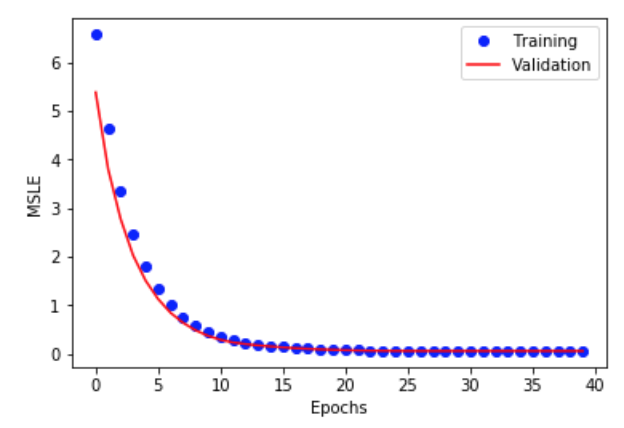
\includegraphics[width=0.48\textwidth]{model_1_msle.png}}
		\subfigure[The loss on the training set and validation set.]{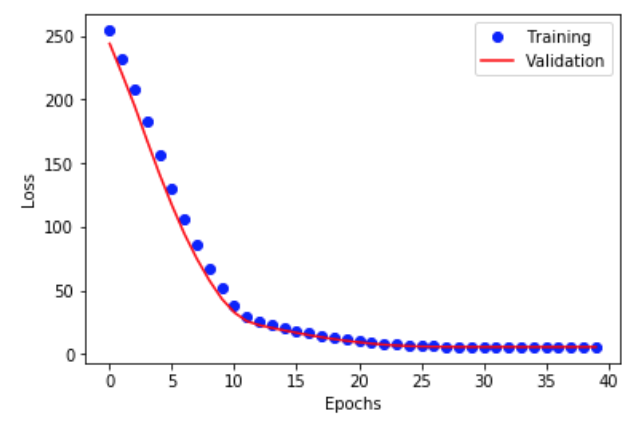
\includegraphics[width=0.48\textwidth]{model_1_loss.png}}
	\end{center}
	\caption{The convergence curves for Model 1.}
	\label{fig:model1}
\end{figure}
\begin{figure}
	\begin{center}
		\subfigure[The MSLE on the training set and validation set.]{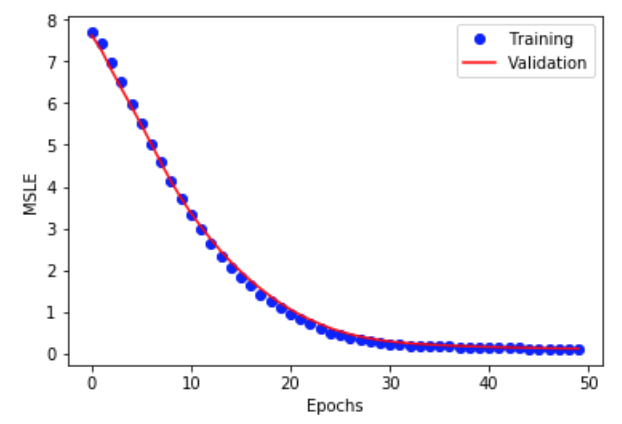
\includegraphics[width=0.48\textwidth]{model_2_msle.png}}
		\subfigure[The loss on the training set and validation set.]{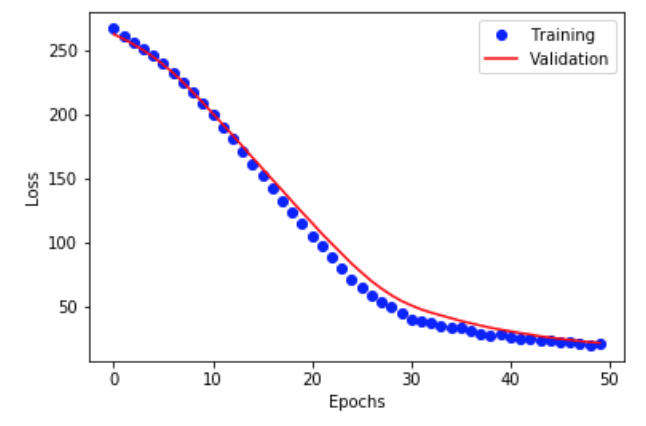
\includegraphics[width=0.48\textwidth]{model_2_loss.png}}
	\end{center}
	\caption{The convergence curves for Model 2.}
	\label{fig:model2}
\end{figure}
\begin{figure}
	\begin{center}
		\subfigure[The MSLE on the training set and validation set.]{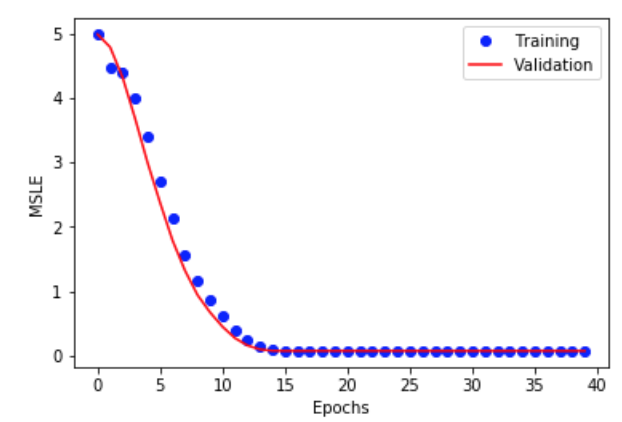
\includegraphics[width=0.48\textwidth]{model_3_msle.png}}
		\subfigure[The loss on the training set and validation set.]{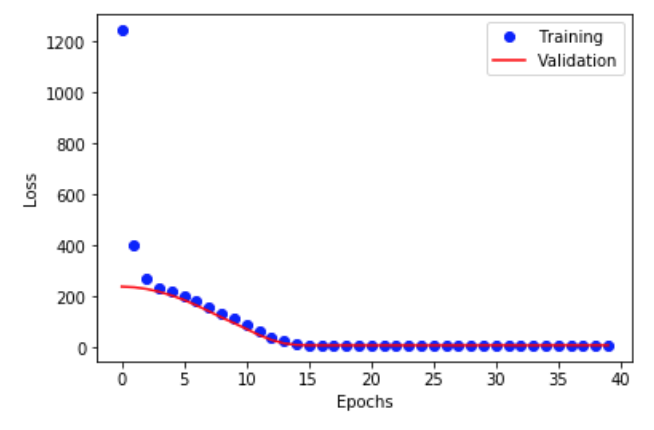
\includegraphics[width=0.48\textwidth]{model_3_loss.png}}
	\end{center}
	\caption{The convergence curves for Model 3.}
	\label{fig:model3}
\end{figure}
\begin{figure}
	\begin{center}
		\subfigure[The heat map for the correlations of all of the different data attributes.]{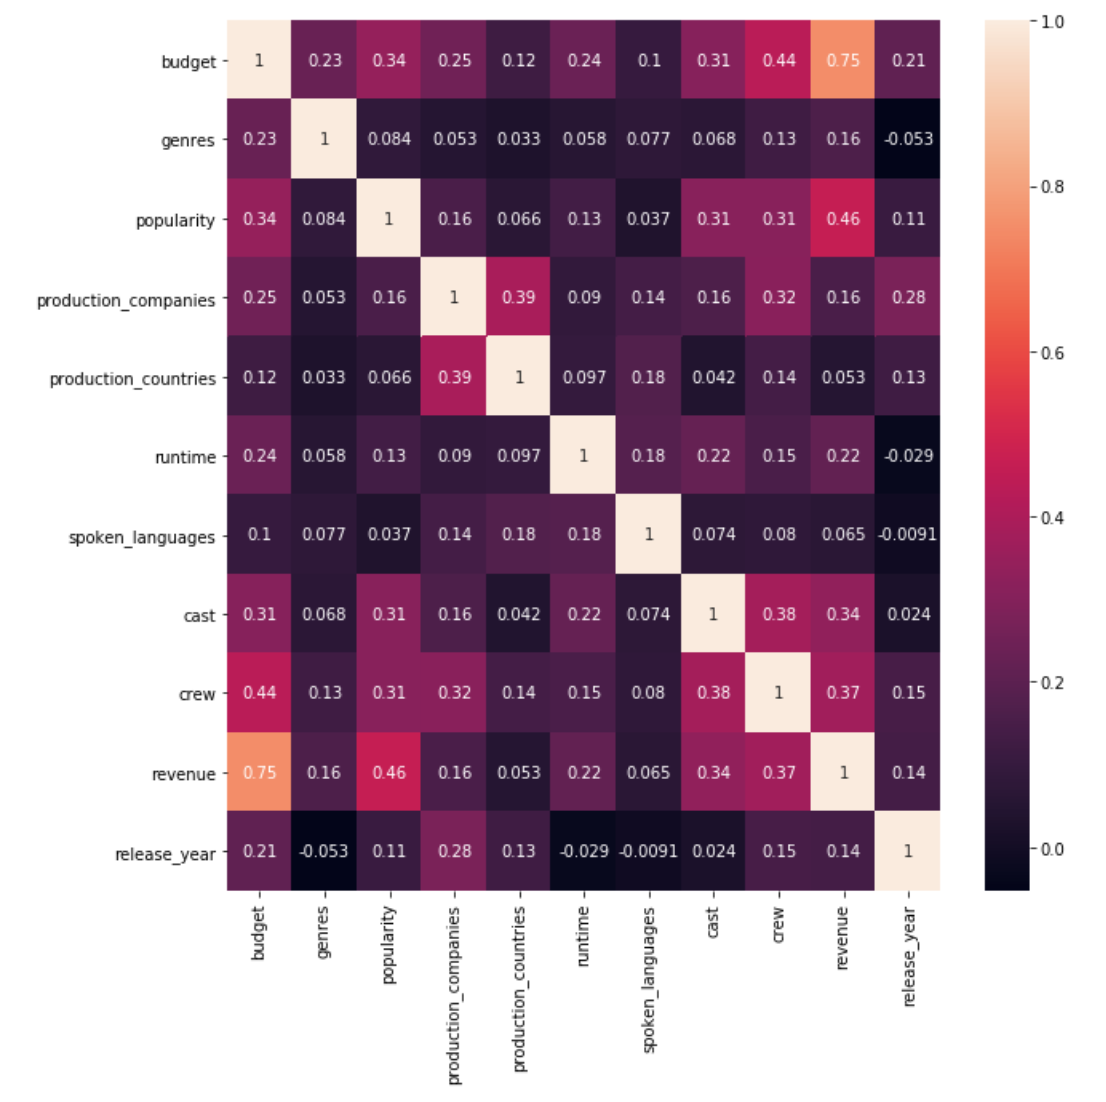
\includegraphics[width=0.75\textwidth]{heatmap.png}}
	\end{center}
	\caption{The heat map for the correlations of all of the different data attributes.}
	\label{fig:heatmap}
\end{figure}
%---------------------------------Figure---------------------------------%

\section{Compared Methods}

As an initial baseline, we simply used a movie's budget and used it as our prediction for the movie's revenue. On Kaggle, this scored a $7.64689$ on the public leaderboard. Our code for this initial baseline can be found at \url{https://github.com/seantrinh/boxoffice/blob/master/baseline.ipynb}.

With our next baseline, we used all of the numerical data of the movie: budget, runtime, and popularity. Using these attributes and feeding them into a model with a few Dense layers produced a score of $2.30819$ on the public leaderboard. Because of its accuracy, this became our first model. 

We then tried to incorporate the number of spoken languages, the number of production companies, the number of production countries, the number of cast members, the number of crew members, and the number of genres, all of which had to be calculated, into the first model. This did not meet our baseline of $2.30819$, only scoring $2.47790$ on the public leaderboard. 

At first, we were not sure why adding in additional data attributes into the model made our score slightly worse. This caused us to perform a thorough analysis on the data, all of which can be found at \url{https://github.com/seantrinh/boxoffice/blob/master/Analysis.ipynb}. We eventually produced a heat map of the correlations between all of the different data attributes. Figure~\ref{fig:heatmap} shows this heat map.

Of particular importance to us was the correlations between the different data attributes and revenue. We saw that our first model performed well because it took into consideration some of the data attributes with the highest correlation to revenue. For example, budget had a $0.75$ correlation to revenue. 

The relatively strong correlations of the number of cast members and the number of crew members to revenue led to the construction of our second model. In addition, in our analysis of release year, we identified a seemingly consistent increase in revenue the later the year. Release month also seemed to have an indication on revenue. This led to the construction of our third model. 

Having tried a couple of times to incorporate these different attributes into one model, we decided to use the predictions of the three models and construct an Ensemble model, described earlier. Doing this resulted in a public score of $2.38089$, an improvement on our previous benchmark. Once we conducted 10-fold cross validation on the models to fine-tune our parameters and trained all of the models and Ensemble model on all of the training data once fine-tuning was complete, we achieved a public score of $2.28782$, another improvement. Although the cross-validation and fine-tuning was completed in other notebooks, which can be found in the same repository, the main code used to produce the CSV file of our submission can be found at \url{https://github.com/seantrinh/boxoffice/blob/master/main.ipynb}.

\section{Other considerations}

\paragraph{Using additional data.}
As mentioned before, one of our challenges was the relatively small amount of data available to use. Because of this, we attempted to locate movie data from other databases and sources. Although data was available, these datasets did not have the same data attributes as the one we were given, making the parsing and addition of this data particularly difficult. Also, the use of additional data was not strictly prohibited, but in the spirit of the competition, participants are asked not to use data outside of the data provided. Because of this, we abandoned this idea.

\paragraph{Using an Embedding layer for text data.}
Our models do not take advantage of a lot of the data attributes containing text, and we knew that we could make improvements to our score if we could incorporate this data. Because of this, we attempted to construct a fourth model to incorporate into our Ensemble model. We used an Embedding layer and Dense layers to construct this fourth model. We then trained and fine-tuned the parameters of this model and incorporated it into our Ensemble model. This, however, produced a public score of $3.41863$, making our prediction more inaccurate. Because of this, we decided not to include this model. The code and results of this fourth model can be found in the repository, towards the bottom of the 'boxoffice' notebook.

\section{Outcome}

We participated in an active competition on Kaggle. Our score on the public leaderboard is $2.28782$. At the time of this writing, our rank on the public leaderboard is 641 out of 1189 teams. Since this is still an ongoing, active competition, we do not yet have a rank nor score on the private leaderboard. 
The screenshot is in Figure~\ref{fig:leaderboard}. The CSV file that was submitted to obtain the public score of $2.28782$ can be found at \url{https://github.com/seantrinh/boxoffice/blob/master/submissions/submission_2-28782.csv}.

%---------------------------------Figure---------------------------------%
\begin{figure}
	\begin{center}
		\subfigure[Public leaderboard.]{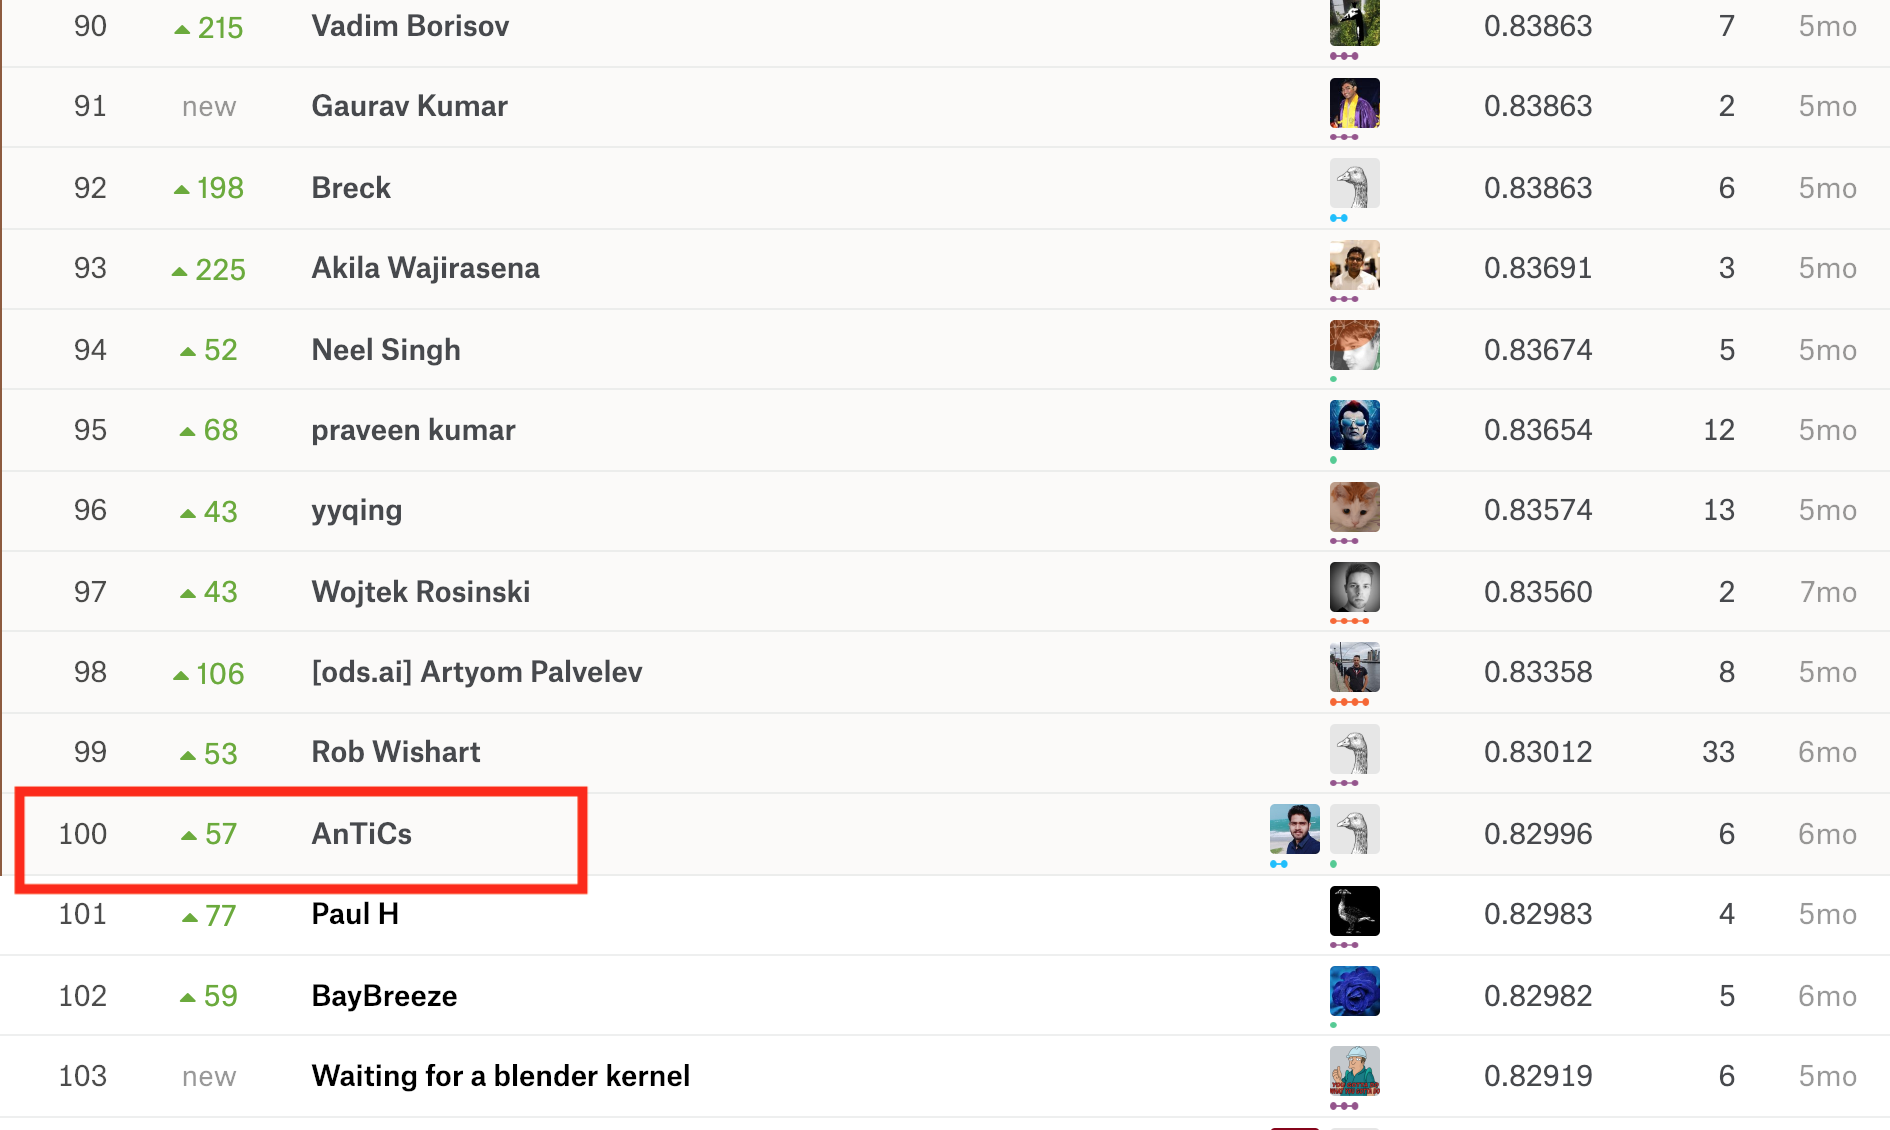
\includegraphics[width=0.75\textwidth]{public.png}}
	\end{center}
	\caption{Our ranking in the public leaderboard.}
	\label{fig:leaderboard}
\end{figure}
%---------------------------------Figure---------------------------------%



%\vspace{3mm}
%\begin{lstlisting}
%import numpy
%
%def rfm(x, s, sigma):
%	n, d = x.shape
%	a = numpy.random.standard_normal((d, s)) / sigma
%	b = numpy.random.rand(1, s) * (2 * numpy.pi)
%	c = numpy.dot(x, a) + b
%	h = numpy.cos(c) * numpy.sqrt(2/s)
%	return h
%\end{lstlisting}
%\vspace{3mm}

%\newpage
\bibliographystyle{plain}
\bibliography{reference}


\end{document}
